\lhead{\textbf{Basic Algorithms, Fall 2024 \\ CSCI-UA.0310-001}}
\chead{\Large{\textbf{Homework 11}}}
\def\lc{\left\lceil}   
\def\rc{\right\rceil}
\newtheorem{claim}{Claim}
\newtheorem{property}{Property}
\rhead{\textbf{Instructor: Rotem Oshman \\ Name: Ishan Pranav}}
\runningheadrule
\firstpageheadrule
\cfoot{}
\stepcounter{subsection}
\section*{References}
Collaborated with Crystal Huang.
\subsection{Prim and Kruskal}
\begin{figure}[h]
    \centering
    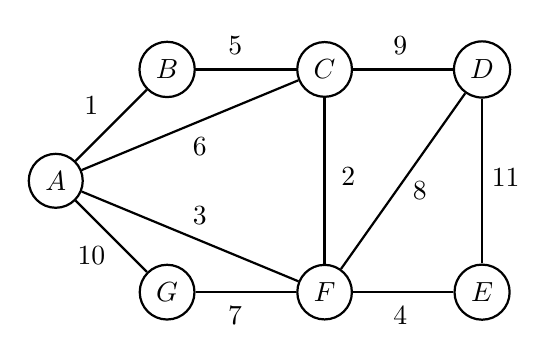
\begin{tikzpicture}[node distance={20mm}, thick,main/.style={circle, thick,draw,font=\sffamily\bfseries}, ar/.style={-{Stealth[scale=1.2]}}]
      \node[main] (1) {$A$}; 
      \node[main] (2) [above right of=1]{$B$};
      \node[main] (3) [right of=2]{$C$};
      \node[main] (4) [right of=3]{$D$};
      \node[main] (5) [below right of=1]{$G$};
      \node[main] (6) [right of=5]{$F$};
      \node[main] (7) [right of=6]{$E$};
      
      \draw (1) -- (2) node [at start, xshift=0.2cm, yshift=0.7cm]{$1$};
      \draw (1) -- (3) node [at start, xshift=1.5cm, yshift=0.3cm]{$6$};
      \draw (1) -- (5) node [at start, xshift=0.2cm, yshift=-0.7cm]{$10$};
      \draw (1) -- (6) node [at start, xshift=1.5cm, yshift=-0.3cm]{$3$};
      \draw (2) -- (3) node [at start, xshift=0.5cm, yshift=0.3cm]{$5$};
      \draw (3) -- (4) node [at start, xshift=0.6cm, yshift=0.3cm]{$9$};
      \draw (3) -- (6) node [at start, xshift=0.3cm, yshift=-1.0cm]{$2$};
      \draw (4) -- (7) node [at start, xshift=0.3cm, yshift=-1.0cm]{$11$};
      \draw (5) -- (6) node [at start, xshift=0.5cm, yshift=-0.3cm]{$7$};
      \draw (6) -- (7) node [at start, xshift=0.6cm, yshift=-0.3cm]{$4$};
      \draw (6) -- (4) node [at start, xshift=1.0cm, yshift=1.0cm]{$8$};
    \end{tikzpicture}
    \caption{\textbf{Undirected graph $\mathbf{G}$.}}
    \label{fig:mst}
\end{figure}

Consider the undirected weighted graph $G = (V, E)$ in Figure~\ref{fig:mst} above.
\begin{enumerate}
    \item  Illustrate a run of Kruskal's algorithm on this graph. State at each step which edge is added to the tree. We have filled the first step in for you. Here, we only want the edge added to the tree and not every edge that is considered. 
    
    \begin{center}
    \begin{tabular}{c|c|c|c|c|c|c|c}
         \textbf{Step} & 1 & 2 & 3 & 4 & 5 & 6\\
         \hline
         \textbf{Edge Added} & $AB$ & $CF$ & $AF$ & $FE$ & $FG$ & $DF$ \\
    \end{tabular}
    \end{center}
\begin{solution}
We can step through Kruskal's algorithm to determine the order of edges added. We sort edges to visit them in descending order of weight and add each vertex to its own set within the disjoint set data structure.

\textit{First. }We consider $AB$. Since $A$ and $B$ are in different sets, we add $AB$ to the tree and merge $A$ and $B$ into a set $AB$.

\textit{Second. }We consider $CF$. Since $C$ and $F$ are in different sets, we add $CF$ to the tree and merge $C$ and $F$ into a set $CF$.

\textit{Third. }We consider $AF$. Since $A$ and $F$ are in different sets, we add $AF$ to the tree and merge $A$ and $F$ into a set $ABCF$.

\textit{Fourth. }We consider $EF$. Since $E$ and $F$ are in different sets, we add $EF$ to the tree and merge $E$ and $F$ into a set $ABCEF$.

\textit{Fifth. }We consider $BC$. Since $B$ and $C$ are in the same set $ABCEF$, we skip this edge.

\textit{Sixth. }We consider $AC$. Since $A$ and $C$ are in the same set $ABCEF$, we skip this edge.

\textit{Seventh. }We consider $FG$. Since $F$ and $G$ are in different sets, we add $FG$ to the tree and merge $F$ and $G$ into a set $ABCEFG$.

\textit{Eighth. }We consider $FD$. Since $F$ and $D$ are in different sets, we add $FD$ to the tree and merge $F$ and $D$ into a set $ABCDEFG$.

\textit{Ninth, tenth, and twelfth. }We consider $CD$, then $AG$, then $DE$. Since $A$, $C$, $D$, $E$, and $G$ are in the same set $ABCDEFG$, we skip these edges.

These steps give the ordering above.
\end{solution}
\item Illustrate a run of Prim's algorithm on this graph starting from vertex $A$. State at each step which edge is added to the tree. We have filled the first step in for you. Here, we only want the edge added to the tree and not every edge that is considered. 

\begin{center}
\begin{tabular}{c|c|c|c|c|c|c|c}
     \textbf{Step} & 1 & 2 & 3 & 4 & 5 & 6\\
     \hline
     \textbf{Edge Added} & $AB$ & $AF$ & $CF$ & $EF$ & $FG$ & $DF$\\
\end{tabular}
\end{center}
\begin{solution}
Stepping through Prim's algorithm to determine the order of edges added by adding edges to a priority queue and extracting the minimum element on each step, we have the ordering above.
\end{solution}
\end{enumerate}
\newpage
\subsection{Minimal spanning tree}
Prove or disprove the following statements. If true, give a short explanation. If false, give a counterexample.

\begin{enumerate}
\item Let $G = (V, E)$ be a connected, undirected graph with a distinct cost $c(e)$ on every edge $e$. Suppose $e^*$ is the cheapest edge in $G$; that is, $c(e^*) < c(e)$ for every edge $e \neq e^*$. Then there is a minimum spanning tree $T$ of $G$ that contains the edge $e^*$.
\begin{solution}

\textbf{Definition I. }Let $G=(V,E)$ be a connected, undirected graph with a distinct cost $c(e)$ for every edge $e\in E$.

\textbf{Definition II. }Let $e^*=\{u,v\}\in E$ be the cheapest edge in $G$; that is, we have $c(e^*)<c(e)$ for all $e\in E$ where $e\neq e^*$.

\textbf{Lemma I. }\textit{Claim. }Let $T=(V,E_T)$ be a spanning tree of $G$ where $e^*\notin E_T$. We can construct a spanning tree of $G$ whose total cost is less than that of $T$.

Since $T$ is a spanning tree of $G$, there exists a path $(u,\dots,x,y,\dots,v)$ in $T$ containing an edge $e'=\{x,y\}$ for $x,y\in V$. Of course, $e'\neq e^*$ since $T$ does not contain $e^*$.

We can add edge $e^*$ to $T$ to construct $T'=(V,E_T\cup\{e^*\})$, an induced subgraph of $G$. Now there exists a cycle $(u,\dots,x,y,\dots,v,u)$ in $T'$ that contains $e'$. Note that $T'$ is connected because $T$ is a tree, and thus connected.

We can construct $T''=(V,(E_T\cup\{e^*\})\setminus\{e'\})$, an induced subgraph of $G$ derived by replacing $e^*$ with $e'$ in $T$; that is, by removing $e'$ from $T'$.

After severing the edge $e'=\{x,y\}$, paths $(x,\dots,u)$ and $(v,\dots,y)$ still do exist in $T''$. Since edge $e^*=\{u,v\}$ does exist in $T''$, there exists a path $(x,\dots,u,v,\dots,y)$ in $T''$. All other vertices in $T''$ are connected because $T'$ is connected. So $T''$ is connected. 

Without $e'=\{x,y\}$, the cycle $(u,\dots,x,y,\dots,v,u)$ does not exist in $T''$. By construction, this is the only cycle in $T''$ since $T$ is a tree, and thus, acyclic. Thus, $T''$ is acyclic.

By construction of $T''$, the total cost of all edges in $T''$ is the total cost of all edges in $T$, minus the cost of $e'$, plus the cost of $e^*$. Since $c(e^*)$ is the cheapest edge in $G$, and $e'\in G$, we know $c(e^*)<c(e')$. Therefore, the total cost of all edges in $T''$ is less than that of all edges in $T$.

Since $T''$ is a connected, acyclic, induced subgraph of $G$ containing all vertices in $G$, we know that $T''$ is a spanning tree. $T''$ is a spanning tree of $G$ with a smaller total cost than $T$---what was to be constructed.

\textbf{Proposition I. }\textit{Claim. }There exists a minimum spanning tree of $G$ that contains $e^*$.

\textit{Proof. }Assume, for the sake of contradiction, that there exists no minimum spanning tree of $G$ that contains edge $e^*=\{u,v\}$ for $u,v\in V$. Since $G$ is connected and undirected, there must exist $T=(V,E_T)$, a minimum spanning tree of $G$. It follows from our hypothesis that $e^*\notin E_T$.

From Lemma I, since $T$ is a spanning tree of $G$ that does not contain its cheapest edge $e^*$, we can construct a spanning tree of $G$ whose total cost is less than that of $T$.

This is absurd: It contradicts the hypothesis that $T$ is a \textit{minimum} spanning tree of $G$. Ergo, the hypothesis is false: There does exist a minimum spanning tree of $G$ containing $e^*.~\square$
\end{solution}
\newpage
\item In the above setting, every MST of $G$ contains the edge $e^*$.
\begin{solution}
\textbf{Proposition II. }\textit{Claim. }Every minimum spanning tree of $G$ contains $e^*$.

\textit{Proof. }Assume, for the sake of contradiction, that there exists some minimum spanning tree $T=(V,E_T)$ of $G$ where $e^*\notin E_T$.

From Lemma I, since $T$ is a spanning tree of $G$ that does not contain its cheapest edge $e^*$, we can construct a spanning tree of $G$ whose total cost is less than that of $T$.

This is absurd: It contradicts the hypothesis that $T$ is a \textit{minimum} spanning tree of $G$. Ergo, the hypothesis is false: Every minimum spanning tree of $G$ does contain $e^*.~\square$
\end{solution}
\newpage
\end{enumerate}
\subsection{Faster minimal spanning tree}
\begin{enumerate}
\item Assume that all edge weights of the given undirected graph $G = (V, E)$ are promised to be $1$. Design the fastest algorithm you can to compute the minimum spanning tree (MST) of $G$. Argue the correctness of the algorithm and state its run-time.
\begin{solution}

\textbf{Algorithm I. }{\sc SpanningTree}($G$) with undirected graph $G=(V,E)$ where all edges have cost 1; returns a minimum spanning tree of $G$:

Let $T\leftarrow\emptyset$.

If $V=\emptyset$, then return $T$.

Let $s\leftarrow v\in V$, choosing $s$ arbitrarily.

For $u\in V$:
\begin{itemize}
    \item assign $u.\mathsf{color}\leftarrow\mathsf{white}$;
    \item assign $u.\mathsf{parent}\leftarrow\mathsf{nil}$.
\end{itemize}

Perform {\sc DepthFirstSearch--Visit}($G,s$); here {\sc DepthFirstSearch--Visit} is the well-known inner loop of the depth-first-search algorithm that visits each vertex in a graph once beginning from a source $s\in V$ and assigns $u.\mathsf{parent}$ to some vertex $v\in V$ for each $u\in V\setminus\{s\}$. Note {\sc DepthFirstSearch--Visit} has running time $O(|V|+|E|)$.

For $v\in V\setminus\{s\}$:
\begin{itemize}
\item if $v.\mathsf{parent}=\sf{nil}$, then throw an error indicating that there exists no spanning tree of $G$;
\item assign $T\leftarrow T\cup\{\{v.\mathsf{parent},v\}\}$.
\end{itemize}

Return $T$.

\textbf{Proposition III. }\textit{Claim. }{\sc SpanningTree}($G$) returns a minimum spanning tree of $G$.

\textit{Proof. }{\sc DepthFirstSearch--Visit} visits each element once and assigns $u.\mathsf{parent}$ to the vertex from which $u$ was reached in the depth-first traversal. By following these parent references, we can traverse the depth-first forest.
\begin{itemize}
\item Suppose that not all vertices are visited by {\sc DepthFirstSearch--Visit}. Then, after the invocation of {\sc DepthFirstSearch--Visit}, there exists some unvisited vertex $v\in V$ where $v\neq s$ but $v.\mathsf{parent}=\mathsf{nil}$. In this case, the depth-first forest has several components, so $G$ is not connected, and thus, a spanning tree does not exist. Algorithm I correctly raises an error.
\item Suppose instead that for all vertices $v\in V\setminus\{s\}$ we have $v.\mathsf{parent}\neq\mathsf{nil}$. This implies that the depth-first forest is in fact a depth-first tree. For each vertex $v\in V\setminus\{s\}$, we insert an edge linking $v.\mathsf{parent}$ to $u$ into our working spanning tree $T$. This process explicitly reconstructs the depth-first tree, which is known to be connected and acyclic. Based on the invocation of {\sc DepthFirstSearch--Visit}, vertex $s$ is the ultimate ancestor in the depth-first tree. The loop body visits all other vertices, which are descendants of $s$. All vertices $u\in V$ are included in $T$ by construction. So $T$ is a spanning tree of $G$.
\end{itemize}
For all edges $e\in E$, the cost of $e$ is 1. By definition, a spanning tree of $G$ has $|V|$ vertices and $|E|=|V|-1$ edges. Thus all spanning trees of $G$ have total cost $|V|-1$, so a spanning tree of $G$ is a minimum spanning tree of $G$. Ergo $T$ is a minimum spanning tree of $G.~\square$

\textbf{Proposition IV. }\textit{Claim. }{\sc SpanningTree}($G$) has running time $O(|V|+|E|)$.

\textit{Proof. }First, Algorithm I invokes {\sc DepthFirstSearch--Visit} with running time $O(|V|+|E|)$.

Then, for each of the $|V|-1$ vertices in $V\setminus\{s\}$, it inserts an edge into $T$ via adjacency list, an $O(1)$ operation. Thus, the running time of the loop is $O(|V|)$.

Finally, Algorithm I returns the resulting tree, an $O(1)$ operation.

Thus, the running time of {\sc SpanningTree}($G$) is $O(|V|+|E|)+O(|V|)=O(|V|+|E|).~\square$
\end{solution}
\newpage
\item Suppose instead that all edge weights are 1 \emph{except} for a single edge $e_0 = (u_0, v_0)$ whose weight is $w_0$ (note, $w_0$ might be either larger or smaller than 1). Show how to modify your solution in part 1 to compute the MST of $G$. What is the running time of your algorithm and how does it compare to the runtime you obtained in part 1 (or standard Prim)?
\begin{solution}

\textbf{Algorithm II. }{\sc SpanningTree2}($G$) with undirected graph $G=(V,E)$ where all edges have cost $1$; returns a minimum spanning tree of $G$:

Let $T\leftarrow\emptyset$.

If $V=\emptyset$, then return $T$.

For $u\in V$:
\begin{itemize}
    \item assign $u.\mathsf{color}\leftarrow\mathsf{white}$;
    \item assign $u.\mathsf{parent}\leftarrow\mathsf{nil}$.
\end{itemize}

Let $\{u_0,v_0\}\leftarrow\mathsf{nil}$.

For $\{u,v\}\in E$:
\begin{itemize}
    \item if $w(u,v)\neq 1$, then:
    \begin{itemize}
        \item assign $\{u_0,v_0\}\leftarrow\{u,v\}$;
        \item break iteration.
    \end{itemize}
\end{itemize}

Let $(a_1,\dots,a_n)$ denote the $n$-element adjacency list of $u_0$.

For $i=1$ to $n$:
\begin{itemize}
\item if $w(u_0,a_i)>1$, then:
\begin{itemize}
    \item swap $a_i$ with $a_n$;
    \item break iteration;
\end{itemize}
\item if $w(u_0,a_i)<1$, then:
\begin{itemize}
    \item swap $a_i$ with $a_1$;
    \item break iteration.
\end{itemize}
\end{itemize}
Perform {\sc DepthFirstSearch--Visit}($G,u_0$); here {\sc DepthFirstSearch--Visit} is the inner loop of the well-known depth-first-search algorithm that visits each vertex in the adjacency list of source $u_0\in V$ and assigns $u.\mathsf{parent}$ to some vertex $v\in V$ for each $u\in V\setminus\{u_0\}$. Note {\sc DepthFirstSearch--Visit} has running time $O(|V|+|E|)$.

For $v\in V\setminus\{u_0\}$:
\begin{itemize}
\item if $v.\mathsf{parent}=\sf{nil}$, then throw an error indicating that there exists no spanning tree of $G$;
\item assign $T\leftarrow T\cup\{\{v.\mathsf{parent},v\}\}$.
\end{itemize}

Return $T$.

\textbf{Proposition V. }\textit{Claim. }{\sc SpanningTree2}($G$) returns a minimum spanning tree of $G$.

\textit{Proof. }{\sc SpanningTree2} is a variant of {\sc DepthFirstSearch}. Using a similar argument to that of Proposition III, we know that $T$ is a spanning tree of $G$. If not, the depth-first forest has several components, so $G$ is not connected, and thus, a spanning tree does not exist. Algorithm II correctly raises an error in that case.

There are two cases: Either $\{u_0,v_0\}$ is a ``heavy'' edge---that is, $w(u_0,v_0)>1$---or a ``light'' edge with $w(u_0,v_0)<1$.

\begin{itemize}
    \item Suppose that $w(u_0,v_0)>1$. Our depth-first search begins from $u_0$ and visits its outgoing edges in ascending order of cost. We either include edge $\{u_0,v_0\}$, or not.
    \begin{itemize}
        \item Suppose $\{u_0,v_0\}\in T$. We sorted the adjacency list of $u_0$ such that $v_0$ is the last child visited. This means there is no other path from $u_0$ to $v_0$ in $G$. Then $T$ is the only spanning tree of $G$, so $T$ is minimal.
        \item Suppose instead $\{u_0,v_0\}\notin T$. Since $T$ is a spanning tree of $G$, we know that $T$ contains $|V|-1$ edges. Since $\{u_0,v_0\}\notin T$, every edge in $T$ has weight $1$. This implies that $T$ has a total cost $|V|-1$. There is no edge in $G$ with a total cost less than $1$, so the minimal spanning tree of $G$ has cost $|V|-1$. Ergo, $T$ is minimal.
    \end{itemize}
    \item Suppose instead that $w(u_0,v_0)<1$. Then, since our depth-first search begins from $u_0$ and visits outgoing edges in ascending order of cost, we include edge $e_0=\{u_0,v_0\}$ always. We know that $e_0$ is the cheapest edge in $G$; that is, for all $e\in E$, we have $w(e_0)<w(e)$. Note that from Proposition II, all minimum spanning trees contain $e_0$.
    
    Since all other edges have weight $1$ and all spanning trees have $|V|-1$ edges, the total cost of any other spanning tree is $|V|-1$. However, since $\{u_0,v_0\}\in T$ has $w(u_0,v_0)<1$, we know that the total total cost of the $|V|-1$ edges in $T$ is less than $|V|-1$. Therefore, $T$ is minimal.
\end{itemize}
In all cases, $T$ is a minimum spanning tree of $G$, so Algorithm II is correct.$~\square$

\textbf{Proposition VI. }\textit{Claim. }{\sc SpanningTree2}($G$) has running time $O(|V|+|E|)$.

\textit{Proof. }First, we initialize the state for each vertex in $V$, which is an $O(|V|)$ process.

Then, we perform a linear search over the edges in $E$ to find $e_0$, which is an $O(|E|)$ process.

We sort the adjacency list of $u_0$ by swapping $e_0$ into its correct position. This operation is linear with respect to the adjacency list of $u_0$. Of course, in the worst case this process is $O(|V|-1)$ if there is an edge connecting $u_0$ to each other vertex in $|V|$.

Invoking {\sc DepthFirstSearch--Visit} is known to be an $O(|V|+|E|)$ process.

Finally, visiting the vertices in $V\setminus\{u_0\}$ to reconstruct the tree is an $O(|V|-1)$ process.

We conclude that {\sc SpanningTree2}($G$) has running time $O(|V|+|E|)$, which is equal to that of Algorithm I. Depending on $|V|$ and $|E|$, Algorithm II performs better than Prim's algorithm. Note that for connected graphs $O(|V|+|E|)=O(|E|\log|V|)$, so the running time of Algorithm II is, asymptotically, no worse than that of Prim's algorithm.$~\square$
\end{solution}
\end{enumerate}